% !TEX root = ../thesis.tex
\chapter{Movish system background}
\label{chapter:movish_system_background}

\section{Introduction}
\label{sec:movish_introduction}

In this chapter the reader can understand the basic architecture of Movish. Since implementing a recommendation system is a challenging process the reader will be guided through all the problems encountered and will receive explanations in how those issues have been addressed either by design or by system architecture in Movish. This chapter is thus fundamental to all the readers that want to understand the basic functions and architecture of the system.
We will start from the basic systems that inspired Movish: ContentWise and Milo. We will analyze Movish itself later on.

\section{ContentWise}
\label{sec:contentwise}

ContentWise is a well known recommendation system developer by the \ac{DEI} of Politecnico di Milano university. This product basically exposed a movie catalog and makes the use able to perform ratings and obtain recommendations using different algorithms. The user is able to change the recommendation system by itself and the interface is designed to be used by recommendation system professionals. The figure \ref{fig:contentwise} shows ContentWise home page.    

\begin{figure}
  \centering
  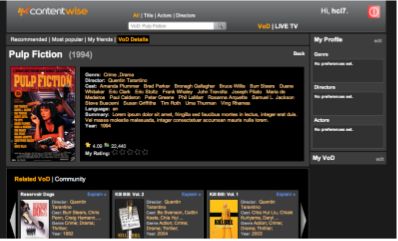
\includegraphics[width=0.9\textwidth]{figures/contentwise-homepage.png}
  \caption{ContentWise}
  \label{fig:contentwise}
\end{figure}

From a first look it is clear that the \ac{GUI} has a late 90' style. The architecture of ContentWise is also very rigid: the algorithms are embedded in the \ac{GUI} and this makes the action of adding a new algorithm really troublesome.
The application is mainly written in Java programming language.

The inability of adding a new algorithm easily and the overcomplicated user interface of ContentWise made the system not suitable for a system that is able to research on new algorithms on unaware users.

\section{Milo}
\label{sec:milo}

During the 2011/2012 course of digital and internet television a new recommendation system for movies that wanted to be similar to ContentWise but more modular and flexible such that it was easy to add new algorithms was implemented.

Since there wanted to be clear distinction between the engine and the presentation a \ac{MVC} \cite{mvc} paradigm has been used. Due to the python programming language popularity and emerging web frameworks, it has been chosen as base language. Among all the available frameworks, Pyramid \cite{pyramid} has been selected thanks to its flexibility and easy to use.

In fact Pyramid allows to have a base \ac{MVC} framework skeleton and plug it with all the libraries you need for your application. Also modifying the base components it is easy and suggested by developers to fully satisfy the application needs. In particular Milo had to communicate with a matlab \cite{matlab} based set of algorithms. Thanks to pymatlab \cite{pymatlab}, python is able to talk directly to matlab in a way that reminds a server-client socket communication.

As stated in chapter \ref{chapter:<recommendation_system_state_of_the_art>}, recommendation systems perform recommendations using a model. This model requires a lot of computational power and time. Web applications have a better user experience if they have a lower page load delay instead. To overcome this conflicting needs a asynchronous task manager framework has been integrated to allow the web application to trigger some events that add new tasks. These tasks are thus run on a separate process.

In order to make the administrator able to add unmodified Matlab \cite{matlab} algorithms the pymatlab \cite{pymatlab} library has been used. Pymatlab makes python be able to communicate with matlab via the matlab shell using accessible via a socket like interface. Figure \ref{fig:urm_creation_code} shows a piece of code of the creation of the \ac{URM} from the python side.

\begin{figure}
  \centering
  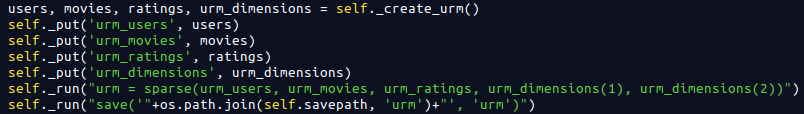
\includegraphics[width=\textwidth]{figures/urm_creation_code.png}
  \caption{URM creation code}
  \label{fig:urm_creation_code}
\end{figure}

The \textit{self.create\_urm()} method generates the urm picking the data from the database. That python function returns a numpy array of users, movies, rating e and array indicating the dimension of the the matrix. The dimension is needed to create a sparse matrix of the right size. In fact the \textit{self.create\_urm()} function only returns actual data, skipping all the zeros. This avoid not necessary usage of ram due to too big matrices. Line from 2 to 5 put the variables in the matlab environment. Line 6 creates the sparse matrix into the matlab environment. The matrix created so is then stored as a .mat file for later use during the creation of the model.

As you can see all the communication is handled by running string like commands. Variables are stored and retrieved from the matlab environment thanks to the \textit{get} and \textit{put} functions of Figure \ref{fig:matlab_put_get_code}.

\begin{figure}
  \centering
  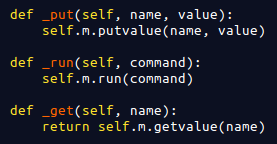
\includegraphics[width=0.4\textwidth]{figures/matlab_put_get_code.png}
  \caption{Code for the python\-matlab communication}
  \label{fig:matlab_put_get_code}
\end{figure}

This allows a clean separation of the python environment and the matlab environment. All the variables are transferred as strings or as floats. This is a limitation of the pymatlab library which is not able to handle integers variable correctly. Also all variables from python to matlab must be numpy \cite{numpy} arrays.

NumPy is the fundamental package for scientific computing with Python. It contains useful function and data structures for easy management of matrices and numerical data arrays. Together with scipy \cite{scipy}, numpy wants to be an open source alternative to matlab providing software for mathematics, science and engineering. Scipy is built on top of numpy.

Milo was developed in a modular way and was the union of two subsystems \cite{thesis-andreia}: a graphical engine and a recommendation engine called Whisperer. Whisperer was in charge of communicating with matlab through the just exposed pymatlab interface. The graphical engine was able to communicate with Whisperer thanks to a rest interface. In order to clarify reader understanding of Milo architecture the user can refer to Figure \ref{fig:milo_architecture}.

\begin{figure}
  \centering
  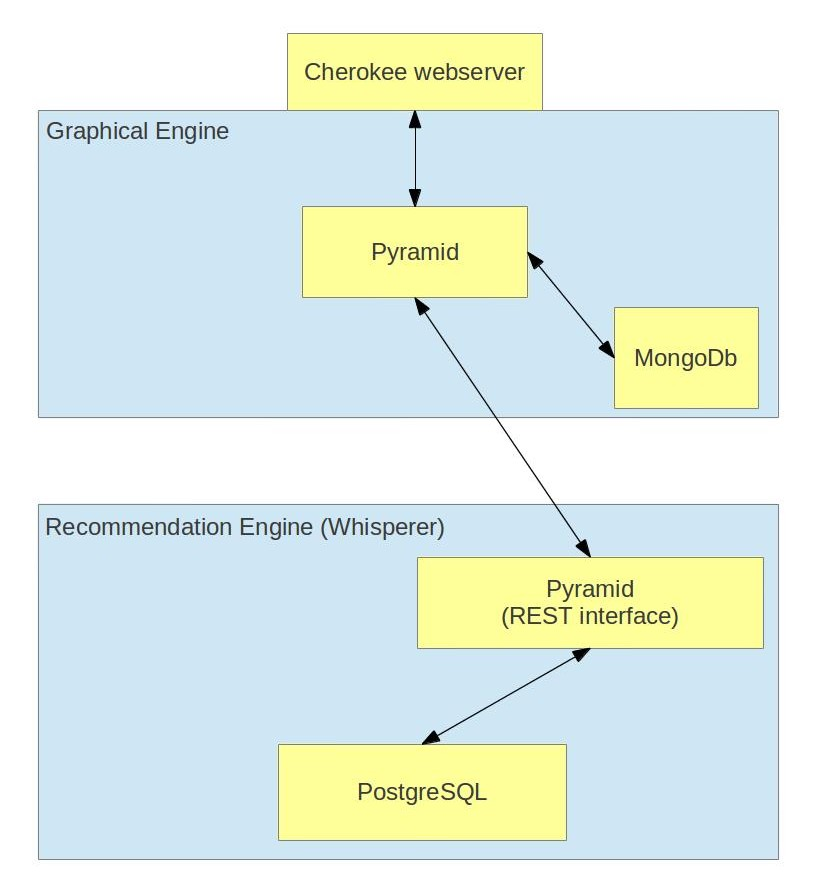
\includegraphics[width=0.7\textwidth]{figures/milo_architecture.jpg}
  \caption{Milo architecture}
  \label{fig:milo_architecture}
\end{figure}

The system is composed by a cherokee webserver. Each requests that arrives to the webserver spawns a new worker or is assigned to an existing one. Each worker is as instance of pyramid web framework with the application running. The frontend database is based on the NoSQL \cite{nosql} MongoDB \cite{mongodb} databases.

NoSQL is a broad class of database management systems identified by non-adherence to the widely used relational database management system model. NoSQL databases are not built primarily on tables, and generally do not use structured query language for data manipulation. NoSQL database systems are often highly optimized for retrieve and append operations and often offer little functionality beyond record storage (e.g. key, value stores). The reduced run-time flexibility compared to full SQL systems is compensated by marked gains in scalability and performance for certain data models. 

In short, NoSQL database management systems are useful when working with a huge quantity of data when the data nature does not require a relational model. The data can be structured, but NoSQL is used when what really matters is the ability to store and retrieve great quantities of data, not the relationships between the elements. Usage examples might be to store millions of key, value pairs in one or a few associative arrays or to store millions of data records. This organization is particularly useful for statistical or real time analyses of growing lists of elements (such as Twitter posts or the Internet server logs from a large group of users).

When the graphical engine needs to do a recommendation it makes a \ac{http} \ac{RESTful} request to another web application, whisperer, that cares about creating the \ac{ICM}, \ac{URM} and all the data structures needed for the recommendation. The recommendation engine relays on a PostgreSQL \cite{postgresql} database for storing the data for the users and the items. Notice that the recommendation engine has only the concept of users and items, this means that it flexible enough to recommend any kind of item to a user. The fact that it was used for movies is thus just a particular case. This was one of the biggest improvements from ContentWise \cite{ContentWise}. The recommendation system developed could be reused for any kind of recommendation.

The recommendation was exposed to the user through a slider placed on top of the page such that the user was likely to watch the slider for first. This has been accomplished using animations in the slider that capture the user attention. The result can be see in Figure \ref{fig:milo_slider} 

\begin{figure}
  \centering
  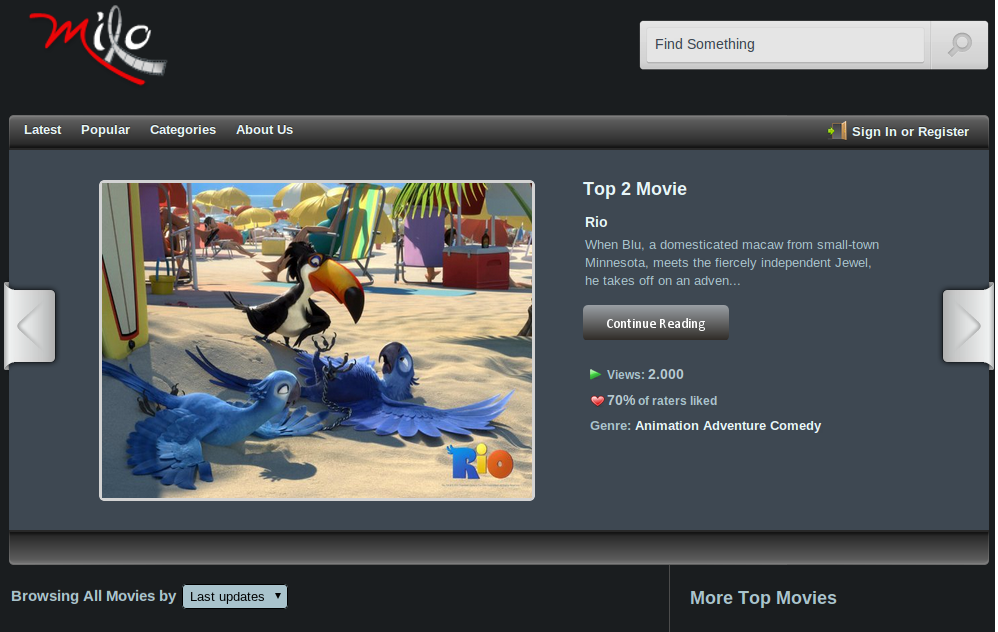
\includegraphics[width=0.7\textwidth]{figures/milo_slider.png}
  \caption{Milo recommendation slider}
  \label{fig:milo_slider}
\end{figure}

The rest of the homepage of Milo can be seen in Figure \ref{fig:milo_homepage}. As studies recall \cite{applicaion-domain-and-functional-classification}, the best way to expose items is an image and a brief description of the item. 

This has been accomplished in milo displaying the cover of the movie, its title, and its genres. Doing so in very few words the user has a clue about the movie and can thus decide if he/she is interested or not in the movie. If the user is interested, he/she can click on the movie cover to have see the movie description shown in Figure \ref{fig:milo_movie} 

\begin{figure}
  \centering
  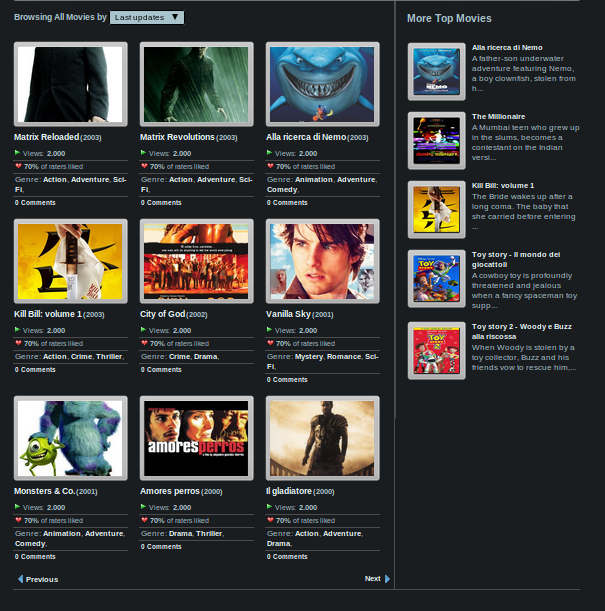
\includegraphics[width=0.7\textwidth]{figures/milo_homepage.png}
  \caption{Milo homepage}
  \label{fig:milo_homepage}
\end{figure}

\begin{figure}
  \centering
  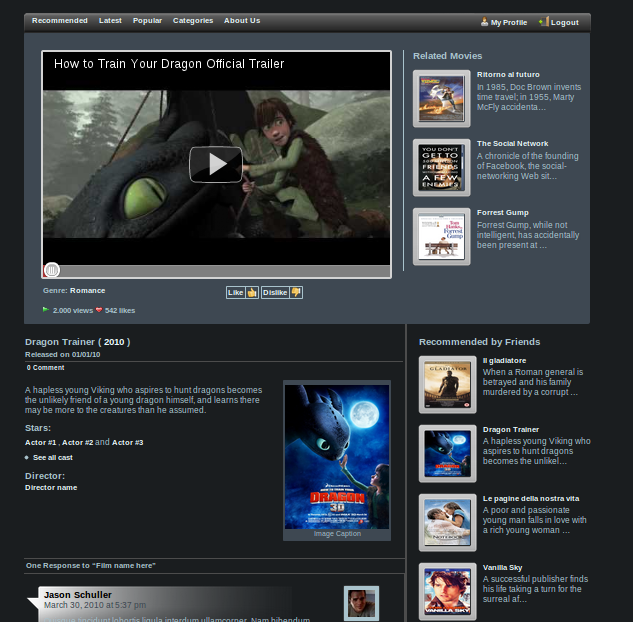
\includegraphics[width=0.7\textwidth]{figures/milo_movie.png}
  \caption{Milo movie description page}
  \label{fig:milo_movie}
\end{figure}

The movie description page is thought to show mainly the poster of the movie in full dimension and its trailer. The user then gets two kinds of recommendation: the content dependent one and a user recommended one using a content based or a user based algorithm that the administrator decided. The user can then read the comments about a movie.

In order to simplify the usage and the administration task, Milo integrated an admin interface to generate the algorithm models, download the relative model files, download the \ac{ICM} and \ac{URM} matrices and manage the surveys. For the first time the admin was able of placing the right matlab file in a directory, load the admin page, create a model for the newly added algorithm and create a survey for that algorithm without modifying one line of code in the system. This was the major improvement of all the previous systems of this kind.

Milo had a two main problems: the first problem was that it had not a clear idea of what it was going to be, that resulted in a hard to maintain code and set of hacks to make things work as fast as possible. This also made the system weak due to many software bottlenecks caused by different databases and mainly by the available hardware for the project that was way limited. Also the matlab part was not optimized in order to reduce memory and free up space as soon as possible. The second problem was mainly the framework chosen, pyramid, that resulted hard to maintain and over complicated in the template section.

Beside those limitations, Milo was an effective and useful system that was able to correctly manage users and generate new surveys.

\section{Movish}
\label{sec:movish}

Movish is a step forward from Milo in the fact that it has a clear vision of the fact that it's a platform for research on new recommendation system algorithms. The system is developed in python and uses web2py \cite{web2py} as main framework. Web2py has been chosen over pyramid because it included all the feature Movish needed:

\begin{itemize}
\item \ac{MVC}. Web2py has a strong \ac{MVC} concept. The structure of the project defines the paths to reach each single function of the application. Models are easy to define thanks to the \ac{DAL} which has a direct mapping to \ac{SQL}. Web2py is also capable of doing automatic migrations: as soon as the code that defines a database table is changed, the application recognizes that and runs a \ac{SQL} ALTER TABLE query to update the database to have the same schema defined by the \ac{DAL}.
The \ac{DAL} code of the database can be seen in Figures \ref{fig:db1}, \ref{fig:db2}, \ref{fig:db3}, \ref{fig:db4}, \ref{fig:db5}. 
The \ac{ER} diagram can be seen on Figure \ref{fig:db_er}. This diagram shows all the relations between the various data structure. The real database is much bigger though. All the data structures used by the web2py framework have been disabled in the graph in order to allow an easy reading of the most important ones.
\item Scheduler. Web2py has a power scheduler built in that has been heavily used in Movish. The use of that component is so deep that I have also found some bugs while coding the various tasks. All bugs promptly reported have been fixed in few days after submission. The scheduler allows the requests to be dispatched as fast as they can while allowing longer tasks to be scheduled. After registering the different tasks the framework itself can also trigger them if some conditions are satisfied. This is heavily used to update movies that have incomplete information.
\end{itemize}

\begin{figure}
  \centering
  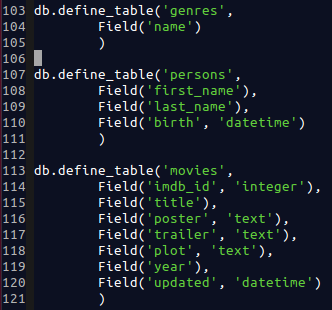
\includegraphics[width=0.7\textwidth]{figures/db1.png}
  \caption{Database definition (part 1)}
  \label{fig:db1}
\end{figure}

\begin{figure}
  \centering
  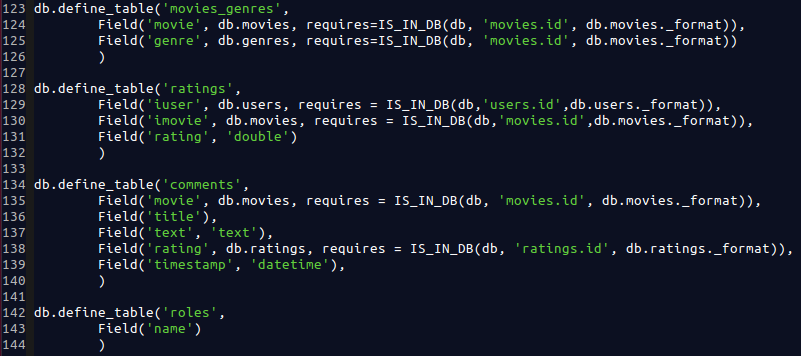
\includegraphics[width=\textwidth]{figures/db2.png}
  \caption{Database definition (part 2)}
  \label{fig:db2}
\end{figure}

\begin{figure}
  \centering
  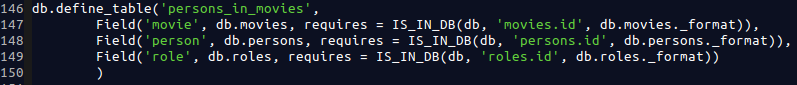
\includegraphics[width=\textwidth]{figures/db3.png}
  \caption{Database definition (part 3)}
  \label{fig:db3}
\end{figure}

\begin{figure}
  \centering
  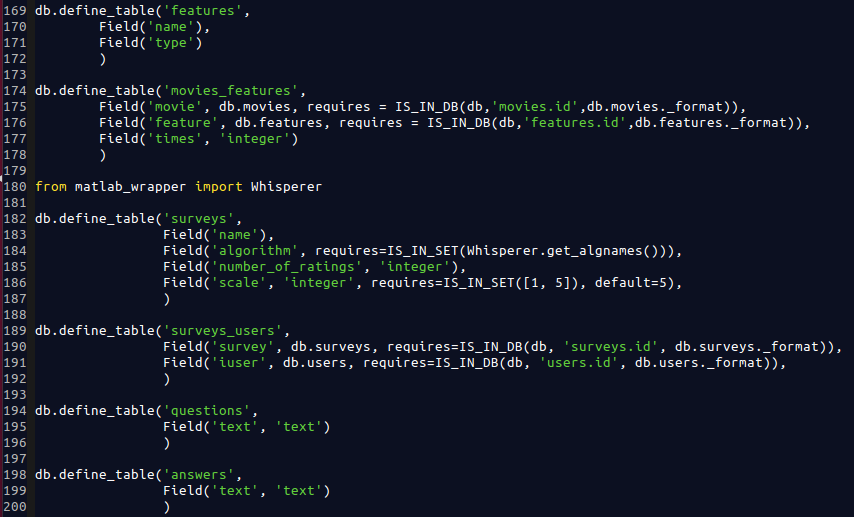
\includegraphics[width=\textwidth]{figures/db4.png}
  \caption{Database definition (part 4)}
  \label{fig:db4}
\end{figure}

\begin{figure}
  \centering
  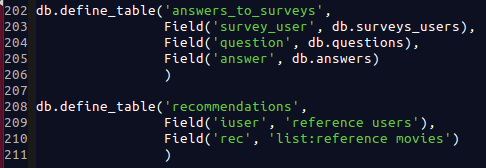
\includegraphics[width=\textwidth]{figures/db5.png}
  \caption{Database definition (part 5)}
  \label{fig:db5}
\end{figure}

The main data structures are the one for storing information about the user called \textit{auth\_user} and \textit{users}, the one for storing the movies called \textit{movies} and the one for the \textit{surveys}. \textit{auth\_user} is web2py specific while \textit{users} is an extension of \textit{auth\_user} in order to support additional field while keeping it separated from the web system. This is so because there are two kind of users in the system. The ones that have registered from the web interface and the ones that have been added from the crawler that gets data from imdb.com \cite{imdb}. We will talk about this later. For now just mind that we don't want to pollute the \textit{auth\_user} table with crawled user that will likely never use the system.

\begin{figure}
  \centering
  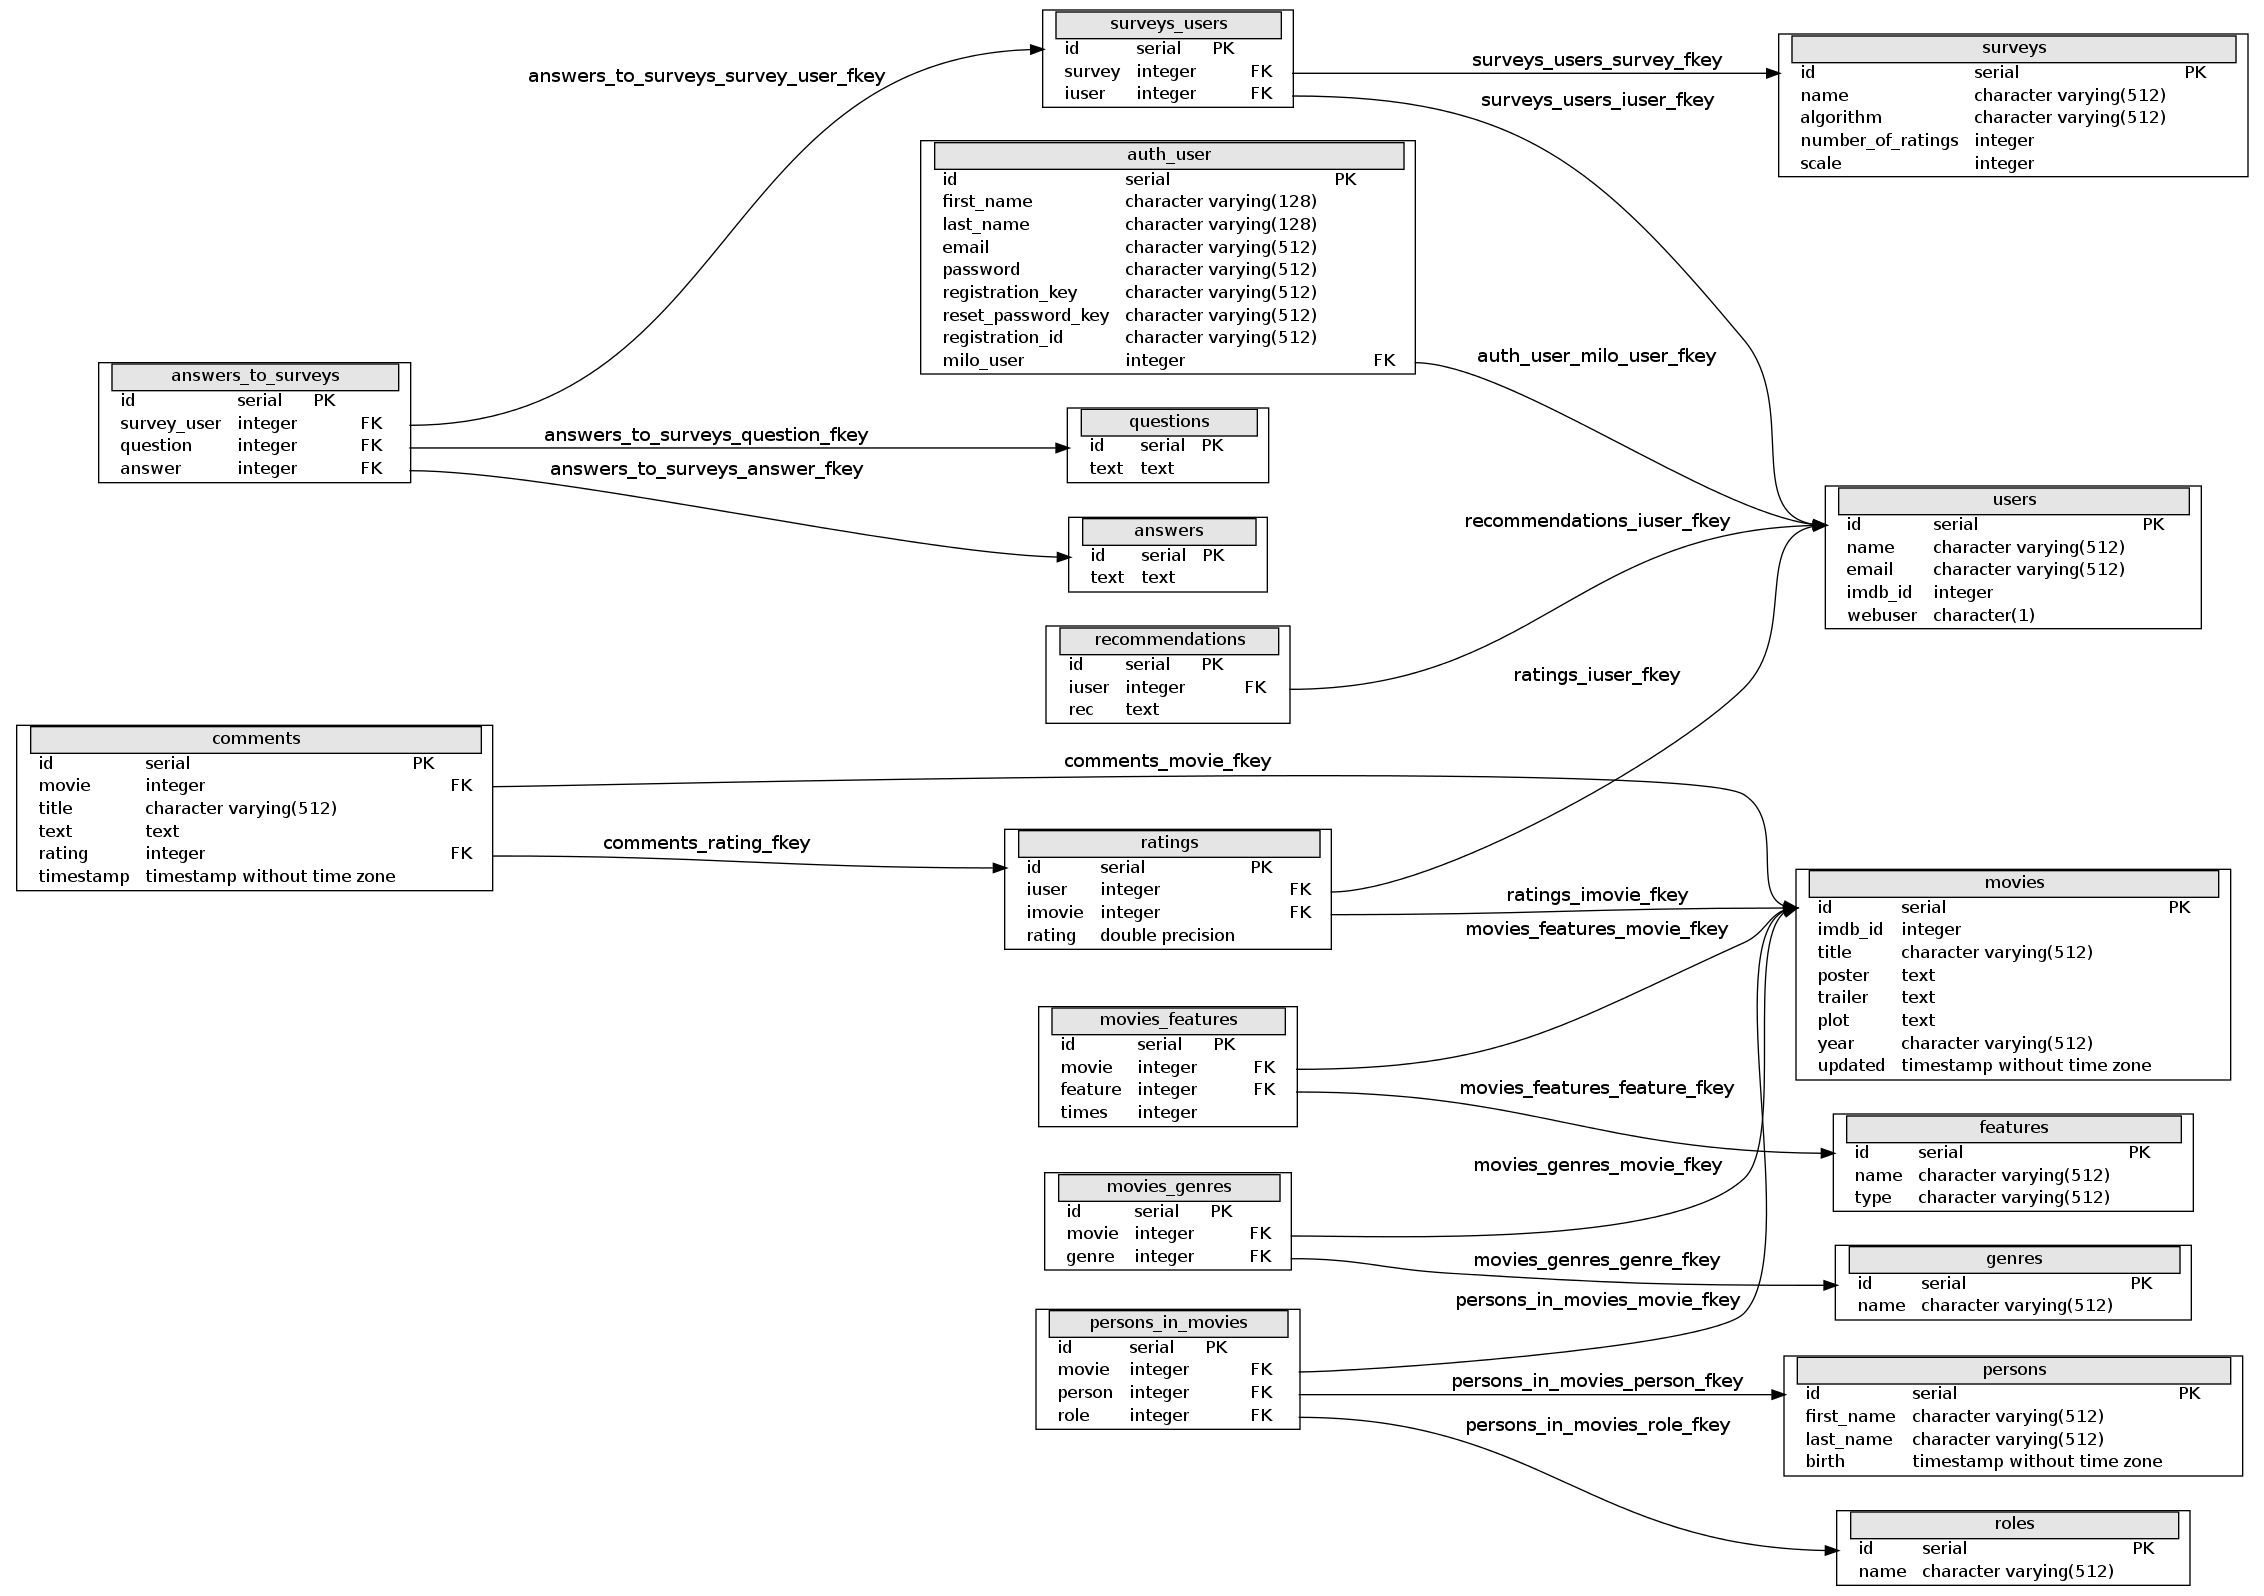
\includegraphics[height=0.7\textheight, angle=90]{figures/db_er.png}
  \caption{Database ER diagram}
  \label{fig:db_er}
\end{figure}

The \textit{movies} data structure stores all the information about a movie and it is i a many-to-many relationship with either \textit{features}, \textit{genres} and \textit{persons\_in\_movies}. \textit{ratings} are also a central data structure that stores all the rating in a relative 0 to 1 float number where 0 is not rated, and 1 is rated as the most awesome movie. Since various algorithms use different scales, this representation allows to use a common scale and then do the required conversion then the \ac{URM} is generated for a particular algorithm.
The \textit{surveys} data structure takes into account the users allowed to perform a survey, the user answers and the algorithm used. The \textit{comments} data structure stores the information about the comments that are associated to a movie and a rating. The \textit{persons\_in\_movies} in Figure \ref{fig:db3} links the persons that can be an actor or a director to a movie. The \textit{recommendations} data structure stores the latest recommendation for a given user and it is the only table that uses the embedded serialization of fields available from \ac{DAL}. In particular storing a list of references in a table like on Figure \ref{fig:db5} it is possible to compress a set of many-to-many entries in a single entry. It is the \ac{DAL} that will care of serializing and deserializing the objects.   
 
As shown in the previous figures the \ac{DAL} makes really easy to define new tables using the \textit{db.define\_table} function which accept the table name as first parameter and then a variable number of Field objects. The Field object take at least one parameter which is the name of the field and optionally a type which describes the kind of data. The data can be of the following types: string, text, blob, boolean, integer, double, decimal, date, time, datetime, password, upload, reference, list:string, list:integer, list:reference, bigint, big-id, big-reference.

As stated before, one of the main advantages of Movish is the heavy use of the scheduler in order to:

\begin{itemize}
\item \textbf{Update the dataset}. It can be updated in two ways: by administrator action or automatically. The administrator can perform the update of all the dataset or import the most popular movies of imdb.com, the coming soon movies or in cinema now movies by clicking the corresponding button in the admin panel. The click will add a task to the scheduler that as soon as it detects a free worker will assign the task. While a movie is displayed, if there are not enough information about that movie, the system automatically generates a task to update that movie. 
  \begin{figure}
    \centering
    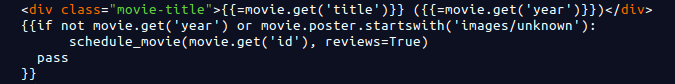
\includegraphics[width=\textwidth]{figures/schedule_autoupdate.png}
    \caption{Schedule movie update code}
    \label{fig:schedule_update}
  \end{figure}

The relevant code about the auto update of a movie is in Figure \ref{fig:schedule_update}. It is part of the view which is the last piece of code executed before sending the output back to the user browser. 

Web2py allows to put pure python code into the \ac{html} pages in order to perform any kind of operation and also embed small logic related to the view. This flexibility is used to detect that if the movie has no year set and the poster is set to the default unknown poster which is \textit{images/unknown} then schedule to retrieve a movie by its id and parse all the reviews of the movie in imdb.com.
\item \textit{Create model}. As explained in Chapter \ref{chapter:<recommendation_system_state_of_the_art>}, the creation of a model is an expensive operation. This characteristic allows it to be suitable for a scheduled task. In fact the administrator can create the model for each supported algorithm clicking the associated button in the administrator interface. Alternatively, the model for a single algorithm is generated as soon as a survey is generated to include the new users that may have been added for the survey.
In fact, doing a recommendation for an user which was not in the \ac{URM} at the moment of model creation will cause an error. This is why it is mandatory to schedule a new model for every newly submitted survey that adds new users to the system.
\item \textbf{Create of the \ac{ICM} and \ac{URM}}. The creation of the two matrices is also an expensive query for the database this is why there is also a task for creating and storing them into matlab as a sparse matrices for easy retrieval.
\item \textbf{Features and titles vectors}. For conformity also the two features and title vectors of all the items in the database are created using a task. The titles vector is a simple vector with the id and all the titles of the movies in the database. The features vector lists, for each item in the database all the metadata, or features, for that item.
\item \textbf{Survey creation}. The creation of a survey is composed by different steps: adding of the new users to the system with an auto generated password, the creation of the model, and an informational mail to each user of the survey telling that the survey is ready and that they can login and perform the survey.
\end{itemize}

Another main component of Movish that was missing in previous systems is the presence of a full featured crawler that uses many sources to retrieve all the needed information for a movie. The crawler is build in a modular and extensible way in order to allow the adding of different sources in the future. As from the time this thesis is being written, the crawler supports the following sources: imdb.com \cite{imdb} via imdbpy \cite{imdbpy} library or by raw \ac{html} parsing via the lxml \cite{lxml} library and youtube. 

Imdbpy is a python package useful to retrieve and manage the data of the imdb movie database about movies, people, characters and companies. It is well maintained an documented and saves the duty to parse the imdb pages by hand. Unfortunately it does support imdb users and reviews so in order to get the reviews of the users from imdb also a raw html parser has been implemented using the lxml library.

lxml is the most feature-rich and easy-to-use library for processing XML and HTML in python. Benchmarks available on their website shows that the library performs better than any known library in generating and parsing xml streams. It is also the library suggested by the python community.
Youtube is accessed via the http RESTful api in order to search movie trailers. It simply searches for the title of the movie appending the word \textit{trailer} to it and picks up the first non sponsored result of the search if any.

\subsection{State of the art issues}
\label{sec:state_of_the_art_issues}

In section \ref{sec:Analysis} we discussed about the issues that may affect a recommendation system. Every real world recommendation system has to address those problems. Movish tries to solve them in this way:

\begin{itemize}
\item \textbf{list of metadata}. Movish uses a tagger on the whole plot to retrieve the maximum number of metadata. It only removes all the conjunctions and stopwords.
\item \textbf{cold start}. In Movish the user is forced, during survey mode that will be exposed in chapter \ref{chapter:<survey_management>}, to perform a number of ratings that the administrator set at survey creation.
\item \textbf{recommendation freshness}, thanks to the importer we will analyze on chapter \ref{sec:importer}, Movish answer to this issue being able to automatically fetch new movies from imdb.com including the ratings and thus the system will have new movies with also ratings. This makes the algorithms be able to use the new movies also at model creation even if the movies have never being displayed on Movish.
\end{itemize}

Other issues are algorithm specific and unable to be solved from Movish. Movish goal is to provide the best up to date environment of \ac{URM}, \ac{ICM}, titles and features vector for an algorithm that has to perform a recommendation. 

\section{Conclusions}
\label{sec:movish_conclusions}

Movish is the first fully automatic recommendation system survey platform. It allows to test different algorithms via surveys without editing any source file of the system. It is inspired by ContentWise and Milo but it introduces a completely new flexible architecture to minimize the administrator workload in keeping the system up to date and ready for testing new algorithms. Movish represent a innovative and fresh approach to the problem of an up to date dataset and optimized environment for recommendation generation.

\acresetall